\documentclass[12pt,]{article}
\usepackage{lmodern}
\usepackage{amssymb,amsmath}
\usepackage{ifxetex,ifluatex}
\usepackage{fixltx2e} % provides \textsubscript
\ifnum 0\ifxetex 1\fi\ifluatex 1\fi=0 % if pdftex
  \usepackage[T1]{fontenc}
  \usepackage[utf8]{inputenc}
\else % if luatex or xelatex
  \ifxetex
    \usepackage{mathspec}
  \else
    \usepackage{fontspec}
  \fi
  \defaultfontfeatures{Ligatures=TeX,Scale=MatchLowercase}
\fi
% use upquote if available, for straight quotes in verbatim environments
\IfFileExists{upquote.sty}{\usepackage{upquote}}{}
% use microtype if available
\IfFileExists{microtype.sty}{%
\usepackage{microtype}
\UseMicrotypeSet[protrusion]{basicmath} % disable protrusion for tt fonts
}{}
\usepackage[margin=1in]{geometry}
\usepackage{hyperref}
\hypersetup{unicode=true,
            pdftitle={Frontal cortex-driven glycinergic inhibition of the intralaminar thalamus},
            pdfauthor={Viktor Plattner},
            pdfborder={0 0 0},
            breaklinks=true}
\urlstyle{same}  % don't use monospace font for urls
\usepackage{color}
\usepackage{fancyvrb}
\newcommand{\VerbBar}{|}
\newcommand{\VERB}{\Verb[commandchars=\\\{\}]}
\DefineVerbatimEnvironment{Highlighting}{Verbatim}{commandchars=\\\{\}}
% Add ',fontsize=\small' for more characters per line
\usepackage{framed}
\definecolor{shadecolor}{RGB}{248,248,248}
\newenvironment{Shaded}{\begin{snugshade}}{\end{snugshade}}
\newcommand{\AlertTok}[1]{\textcolor[rgb]{0.94,0.16,0.16}{#1}}
\newcommand{\AnnotationTok}[1]{\textcolor[rgb]{0.56,0.35,0.01}{\textbf{\textit{#1}}}}
\newcommand{\AttributeTok}[1]{\textcolor[rgb]{0.77,0.63,0.00}{#1}}
\newcommand{\BaseNTok}[1]{\textcolor[rgb]{0.00,0.00,0.81}{#1}}
\newcommand{\BuiltInTok}[1]{#1}
\newcommand{\CharTok}[1]{\textcolor[rgb]{0.31,0.60,0.02}{#1}}
\newcommand{\CommentTok}[1]{\textcolor[rgb]{0.56,0.35,0.01}{\textit{#1}}}
\newcommand{\CommentVarTok}[1]{\textcolor[rgb]{0.56,0.35,0.01}{\textbf{\textit{#1}}}}
\newcommand{\ConstantTok}[1]{\textcolor[rgb]{0.00,0.00,0.00}{#1}}
\newcommand{\ControlFlowTok}[1]{\textcolor[rgb]{0.13,0.29,0.53}{\textbf{#1}}}
\newcommand{\DataTypeTok}[1]{\textcolor[rgb]{0.13,0.29,0.53}{#1}}
\newcommand{\DecValTok}[1]{\textcolor[rgb]{0.00,0.00,0.81}{#1}}
\newcommand{\DocumentationTok}[1]{\textcolor[rgb]{0.56,0.35,0.01}{\textbf{\textit{#1}}}}
\newcommand{\ErrorTok}[1]{\textcolor[rgb]{0.64,0.00,0.00}{\textbf{#1}}}
\newcommand{\ExtensionTok}[1]{#1}
\newcommand{\FloatTok}[1]{\textcolor[rgb]{0.00,0.00,0.81}{#1}}
\newcommand{\FunctionTok}[1]{\textcolor[rgb]{0.00,0.00,0.00}{#1}}
\newcommand{\ImportTok}[1]{#1}
\newcommand{\InformationTok}[1]{\textcolor[rgb]{0.56,0.35,0.01}{\textbf{\textit{#1}}}}
\newcommand{\KeywordTok}[1]{\textcolor[rgb]{0.13,0.29,0.53}{\textbf{#1}}}
\newcommand{\NormalTok}[1]{#1}
\newcommand{\OperatorTok}[1]{\textcolor[rgb]{0.81,0.36,0.00}{\textbf{#1}}}
\newcommand{\OtherTok}[1]{\textcolor[rgb]{0.56,0.35,0.01}{#1}}
\newcommand{\PreprocessorTok}[1]{\textcolor[rgb]{0.56,0.35,0.01}{\textit{#1}}}
\newcommand{\RegionMarkerTok}[1]{#1}
\newcommand{\SpecialCharTok}[1]{\textcolor[rgb]{0.00,0.00,0.00}{#1}}
\newcommand{\SpecialStringTok}[1]{\textcolor[rgb]{0.31,0.60,0.02}{#1}}
\newcommand{\StringTok}[1]{\textcolor[rgb]{0.31,0.60,0.02}{#1}}
\newcommand{\VariableTok}[1]{\textcolor[rgb]{0.00,0.00,0.00}{#1}}
\newcommand{\VerbatimStringTok}[1]{\textcolor[rgb]{0.31,0.60,0.02}{#1}}
\newcommand{\WarningTok}[1]{\textcolor[rgb]{0.56,0.35,0.01}{\textbf{\textit{#1}}}}
\usepackage{graphicx,grffile}
\makeatletter
\def\maxwidth{\ifdim\Gin@nat@width>\linewidth\linewidth\else\Gin@nat@width\fi}
\def\maxheight{\ifdim\Gin@nat@height>\textheight\textheight\else\Gin@nat@height\fi}
\makeatother
% Scale images if necessary, so that they will not overflow the page
% margins by default, and it is still possible to overwrite the defaults
% using explicit options in \includegraphics[width, height, ...]{}
\setkeys{Gin}{width=\maxwidth,height=\maxheight,keepaspectratio}
\IfFileExists{parskip.sty}{%
\usepackage{parskip}
}{% else
\setlength{\parindent}{0pt}
\setlength{\parskip}{6pt plus 2pt minus 1pt}
}
\setlength{\emergencystretch}{3em}  % prevent overfull lines
\providecommand{\tightlist}{%
  \setlength{\itemsep}{0pt}\setlength{\parskip}{0pt}}
\setcounter{secnumdepth}{5}
% Redefines (sub)paragraphs to behave more like sections
\ifx\paragraph\undefined\else
\let\oldparagraph\paragraph
\renewcommand{\paragraph}[1]{\oldparagraph{#1}\mbox{}}
\fi
\ifx\subparagraph\undefined\else
\let\oldsubparagraph\subparagraph
\renewcommand{\subparagraph}[1]{\oldsubparagraph{#1}\mbox{}}
\fi

%%% Use protect on footnotes to avoid problems with footnotes in titles
\let\rmarkdownfootnote\footnote%
\def\footnote{\protect\rmarkdownfootnote}

%%% Change title format to be more compact
\usepackage{titling}

% Create subtitle command for use in maketitle
\providecommand{\subtitle}[1]{
  \posttitle{
    \begin{center}\large#1\end{center}
    }
}

\setlength{\droptitle}{-2em}

  \title{Frontal cortex-driven glycinergic inhibition of the intralaminar
thalamus}
    \pretitle{\vspace{\droptitle}\centering\huge}
  \posttitle{\par}
    \author{Viktor Plattner}
    \preauthor{\centering\large\emph}
  \postauthor{\par}
    \date{}
    \predate{}\postdate{}
  

\begin{document}
\maketitle

{
\setcounter{tocdepth}{2}
\tableofcontents
}
\hypertarget{firing-rate-of-il-neurons-during-glycinergic-fiber-activation}{%
\section{Firing rate of IL neurons during glycinergic fiber
activation}\label{firing-rate-of-il-neurons-during-glycinergic-fiber-activation}}

In these experiments glycinergic fibers were photactivated while the
firing rate of individual IL neurons was recorded. Some of the IL cells
had very low baseline activity. In order to increase the firing rate of
the IL neurons and to detect the effect of the glycinergic fiber
activation a small tail pinch was applied. The firing rate of the
recorded IL cells decreased during the glycinergic fiber activation.

\hypertarget{loading-data}{%
\subsection{Loading data}\label{loading-data}}

Loading AP and stimuli times from \emph{stimulus} and from
\emph{baseline} data to \textbf{IL\_stim\_firing} and to
\textbf{IL\_baseline\_firing} tables:

\begin{Shaded}
\begin{Highlighting}[]
\NormalTok{IL_stim_firing <-}\StringTok{ }\KeywordTok{CreateRecTibble}\NormalTok{(}\DataTypeTok{AP_times =} \KeywordTok{read_csv}\NormalTok{(}\KeywordTok{file.path}\NormalTok{(}\StringTok{"data"}\NormalTok{, }
    \StringTok{"IL_MFR"}\NormalTok{, }\StringTok{"stimulus"}\NormalTok{, }\StringTok{"AP_times.csv"}\NormalTok{)), }
    \DataTypeTok{stim_times =} \KeywordTok{read_csv}\NormalTok{(}\KeywordTok{file.path}\NormalTok{(}\StringTok{"data"}\NormalTok{, }
        \StringTok{"IL_MFR"}\NormalTok{, }\StringTok{"stimulus"}\NormalTok{, }\StringTok{"stim_times.csv"}\NormalTok{)))}
\NormalTok{IL_stim_firing }\OperatorTok\StringTok{ }\KeywordTok{head}\NormalTok{()}
\end{Highlighting}
\end{Shaded}

\begin{verbatim}
## # A tibble: 6 x 7
##   file_name animal_id signal_type unit_id signal_time stim_freq
##   <chr>     <chr>     <chr>         <dbl>       <dbl> <chr>    
## 1 cell01_0~ not spec~ AP                1      0.0376 no value 
## 2 cell01_0~ not spec~ AP                1      0.0644 no value 
## 3 cell01_0~ not spec~ AP                1      0.0903 no value 
## 4 cell01_0~ not spec~ AP                1      0.147  no value 
## 5 cell01_0~ not spec~ AP                1      0.200  no value 
## 6 cell01_0~ not spec~ AP                1      0.239  no value 
## # ... with 1 more variable: available_freqs <chr>
\end{verbatim}

\begin{Shaded}
\begin{Highlighting}[]
\NormalTok{IL_baseline_firing <-}\StringTok{ }\KeywordTok{CreateRecTibble}\NormalTok{(}\DataTypeTok{AP_times =} \KeywordTok{read_csv}\NormalTok{(}\KeywordTok{file.path}\NormalTok{(}\StringTok{"data"}\NormalTok{, }
    \StringTok{"IL_MFR"}\NormalTok{, }\StringTok{"baseline"}\NormalTok{, }\StringTok{"AP_times.csv"}\NormalTok{)), }
    \DataTypeTok{stim_times =} \KeywordTok{read_csv}\NormalTok{(}\KeywordTok{file.path}\NormalTok{(}\StringTok{"data"}\NormalTok{, }
        \StringTok{"IL_MFR"}\NormalTok{, }\StringTok{"baseline"}\NormalTok{, }\StringTok{"stim_times.csv"}\NormalTok{)))}
\NormalTok{IL_stim_firing }\OperatorTok\StringTok{ }\KeywordTok{head}\NormalTok{()}
\end{Highlighting}
\end{Shaded}

\begin{verbatim}
## # A tibble: 6 x 7
##   file_name animal_id signal_type unit_id signal_time stim_freq
##   <chr>     <chr>     <chr>         <dbl>       <dbl> <chr>    
## 1 cell01_0~ not spec~ AP                1      0.0376 no value 
## 2 cell01_0~ not spec~ AP                1      0.0644 no value 
## 3 cell01_0~ not spec~ AP                1      0.0903 no value 
## 4 cell01_0~ not spec~ AP                1      0.147  no value 
## 5 cell01_0~ not spec~ AP                1      0.200  no value 
## 6 cell01_0~ not spec~ AP                1      0.239  no value 
## # ... with 1 more variable: available_freqs <chr>
\end{verbatim}

\hypertarget{summary-information}{%
\subsection{Summary information}\label{summary-information}}

Summary information of the \emph{stimulus} and \emph{baseline} recording
files:

\begin{itemize}
\tightlist
\item
  Variables:

  \begin{itemize}
  \tightlist
  \item
    file names (\emph{file\_name})
  \item
    number of channels in the raw recording files (\emph{No\_ch})
  \item
    number of APs (\emph{No\_AP\_unit}, \emph{No\_AP\_unit2})
  \item
    number of stimulus trains (\emph{No\_Stim})
  \item
    LFP sampling rate (\emph{samp\_rate\_lfp})
  \item
    unit sampling rate (\emph{samp\_rate\_unit})
  \item
    length of the recording (\emph{rec\_length})
  \item
    length of the stimulus trains (\emph{No\_trains})
  \item
    Are the lengths of the stimulus trains equal in the recording
    (\emph{train\_length\_equal})
  \item
    starting time of the stimulus trains (\emph{train\_start})
  \item
    ending time of the stimulus trains (\emph{train\_end})
  \end{itemize}
\end{itemize}

\hypertarget{htmlwidget-86ab837c6ef0a33c718d}{}

\hypertarget{htmlwidget-ef282fb4a4e4ffe83a65}{}

\textbf{CELL\_INFO} table to store the cell categories. It was created
manually using the information from the summary excel table
(\emph{Glicy\_juxta-fm\_exp\_records\_injection\_sum.xls})

\begin{itemize}
\tightlist
\item
  Variables

  \begin{itemize}
  \tightlist
  \item
    cell identification (\emph{cell\_id}). To find the recording file
    use the summary excel table
  \item
    file names (\emph{file\_name})
  \item
    spontaneously active cells (\emph{bl\_activity})
  \item
    induced firing (\emph{pinch})
  \item
    individually identified neurons (\emph{ident})
  \item
    control cells (\emph{control})
  \end{itemize}
\end{itemize}

\hypertarget{htmlwidget-a001e3e2cbab664722e2}{}

\hypertarget{calculations}{%
\subsection{Calculations}\label{calculations}}

\hypertarget{firing-rates}{%
\subsubsection{Firing rates}\label{firing-rates}}

\textbf{b\_d\_a\_MFR}: Calculating the number of APs -using a custom
made function (\emph{BDACalculator})- before during and after the
stimulus trains (\emph{b\_d\_a\_MFR}).

\begin{Shaded}
\begin{Highlighting}[]
\NormalTok{b_d_a_MFR <-}\StringTok{ }\KeywordTok{lapply}\NormalTok{(CELL_INFO}\OperatorTok{$}\NormalTok{cell_id, }
\NormalTok{    BDACalculator, }\DataTypeTok{data =}\NormalTok{ IL_stim_firing) }\OperatorTok\StringTok{ }
\StringTok{    }\KeywordTok{bind_rows}\NormalTok{() }\OperatorTok\StringTok{ }\KeywordTok{mutate}\NormalTok{(}\DataTypeTok{FR =}\NormalTok{ No_AP}\OperatorTok{/}\NormalTok{train_length) }\OperatorTok\StringTok{ }
\StringTok{    }\NormalTok{dplyr}\OperatorTok{::}\KeywordTok{group_by}\NormalTok{(stim_cond, }
\NormalTok{        cell_id) }\OperatorTok\StringTok{ }\KeywordTok{summarise}\NormalTok{(}\DataTypeTok{MFR =} \KeywordTok{mean}\NormalTok{(FR))}
\end{Highlighting}
\end{Shaded}

\begin{verbatim}
## Warning: `as.tibble()` is deprecated, use `as_tibble()` (but mind the new semantics).
## This warning is displayed once per session.
\end{verbatim}

\textbf{sd\_mean\_isi}: Calculating the baseline MFR of the recorded IL
cells from the \emph{IL\_baseline\_firing} table using a custom made
function (\emph{SDMeanISI}). The results are stored in the
\emph{sd\_mean\_isi} table.

\hypertarget{ranks-strength-of-inhibition}{%
\subsubsection{Ranks (strength of
inhibition)}\label{ranks-strength-of-inhibition}}

\textbf{cellranks}: Calculating ranks based on the activity change from
``\emph{baseline}'' to ``\emph{during stimulus}''. If the activity
change is negative (decreased MFR) the asigned rank is negative, if it
is positive (increased MFR) the assigned rank is positive.

Calculating the firing rate change during stimulus (photoactivation of
the glycinergic fibers) compared to baseline:

\[\mathbf{activity\_change} = \frac{during\_MFR - base\_MFR}{base\_MFR} * 100\]

\begin{Shaded}
\begin{Highlighting}[]
\NormalTok{cellranks <-}\StringTok{ }\NormalTok{b_d_a_MFR }\OperatorTok\StringTok{ }\KeywordTok{group_by}\NormalTok{(stim_cond) }\OperatorTok\StringTok{ }
\StringTok{    }\KeywordTok{mutate}\NormalTok{(}\DataTypeTok{base_MFR =}\NormalTok{ sd_mean_isi}\OperatorTok{$}\NormalTok{MFR) }\OperatorTok\StringTok{ }
\StringTok{    }\KeywordTok{mutate}\NormalTok{(}\DataTypeTok{activity_change =}\NormalTok{ ((MFR }\OperatorTok{-}\StringTok{ }
\StringTok{        }\NormalTok{base_MFR)}\OperatorTok{/}\NormalTok{base_MFR }\OperatorTok{*}\StringTok{ }\DecValTok{100}\NormalTok{) }\OperatorTok\StringTok{ }
\StringTok{        }\KeywordTok{round}\NormalTok{(}\DecValTok{2}\NormalTok{)) }\OperatorTok\StringTok{ }\NormalTok{dplyr}\OperatorTok{::}\KeywordTok{filter}\NormalTok{(stim_cond }\OperatorTok{==}\StringTok{ }
\StringTok{    "d"}\NormalTok{) }\OperatorTok\StringTok{ }\KeywordTok{mutate}\NormalTok{(}\DataTypeTok{change_rank =} \KeywordTok{ifelse}\NormalTok{(activity_change }\OperatorTok{>}\StringTok{ }
\StringTok{    }\DecValTok{0}\NormalTok{, }\KeywordTok{rank}\NormalTok{(activity_change), }\OperatorTok{-}\KeywordTok{rank}\NormalTok{(}\OperatorTok{-}\NormalTok{activity_change))) }\OperatorTok\StringTok{ }
\StringTok{    }\KeywordTok{ungroup}\NormalTok{() }\OperatorTok\StringTok{ }\KeywordTok{left_join}\NormalTok{(CELL_INFO }\OperatorTok\StringTok{ }
\StringTok{    }\KeywordTok{select}\NormalTok{(cell_id, control, pinch, }
\NormalTok{        position), }\DataTypeTok{by =} \StringTok{"cell_id"}\NormalTok{)}
\NormalTok{cellranks}
\end{Highlighting}
\end{Shaded}

\begin{verbatim}
## # A tibble: 29 x 9
##    stim_cond cell_id   MFR base_MFR activity_change change_rank control
##    <fct>     <chr>   <dbl>    <dbl>           <dbl>       <dbl> <lgl>  
##  1 d         cell01  5.34    25.4            -79.0          -18 FALSE  
##  2 d         cell02  5.86     8.04           -27.1          -12 FALSE  
##  3 d         cell03  0.300    0.311           -3.44          -8 FALSE  
##  4 d         cell04  0.162    1.03           -84.2          -21 FALSE  
##  5 d         cell05  0.729    2.23           -67.4          -16 FALSE  
##  6 d         cell06  2.54    13.8            -81.6          -20 FALSE  
##  7 d         cell07  0.223    1.12           -80.0          -19 FALSE  
##  8 d         cell08  7.97     1.74           357.            28 FALSE  
##  9 d         cell09  0.688    1.59           -56.7          -14 FALSE  
## 10 d         cell10  4.25     5.08           -16.3          -10 FALSE  
## # ... with 19 more rows, and 2 more variables: pinch <lgl>, position <chr>
\end{verbatim}

\textbf{cellranks\_before\_stim}: Calculating ranks based on the
activity change from ``\emph{before stimulus}'' to ``\emph{during
stimulus}''. If the activity change is negative (decreased MFR) the
asigned rank is negative, if it is positive (increased MFR) the assigned
rank is positive.

Calculating the firing rate change during stimulus (photoactivation of
the glycinergic fibers) compared to before stimulus:

\[\mathbf{activity\_change} = \frac{during\_MFR - before\_MFR}{before\_MFR} * 100\]

\begin{Shaded}
\begin{Highlighting}[]
\NormalTok{cellranks_before_stim <-}\StringTok{ }\NormalTok{b_d_a_MFR }\OperatorTok\StringTok{ }
\StringTok{    }\KeywordTok{spread}\NormalTok{(}\DataTypeTok{key =}\NormalTok{ stim_cond, }\DataTypeTok{value =}\NormalTok{ MFR) }\OperatorTok\StringTok{ }
\StringTok{    }\KeywordTok{mutate}\NormalTok{(}\DataTypeTok{activity_change =}\NormalTok{ ((d }\OperatorTok{-}\StringTok{ }
\StringTok{        }\NormalTok{b)}\OperatorTok{/}\NormalTok{b }\OperatorTok{*}\StringTok{ }\DecValTok{100}\NormalTok{) }\OperatorTok\StringTok{ }\KeywordTok{round}\NormalTok{(}\DecValTok{2}\NormalTok{)) }\OperatorTok\StringTok{ }
\StringTok{    }\KeywordTok{mutate}\NormalTok{(}\DataTypeTok{change_rank =} \KeywordTok{ifelse}\NormalTok{(activity_change }\OperatorTok{>}\StringTok{ }
\StringTok{        }\DecValTok{0}\NormalTok{, }\KeywordTok{rank}\NormalTok{(activity_change), }
        \OperatorTok{-}\KeywordTok{rank}\NormalTok{(}\OperatorTok{-}\NormalTok{activity_change))) }\OperatorTok\StringTok{ }
\StringTok{    }\KeywordTok{left_join}\NormalTok{(CELL_INFO }\OperatorTok\StringTok{ }\KeywordTok{select}\NormalTok{(cell_id, }
\NormalTok{        control, pinch, position), }
        \DataTypeTok{by =} \StringTok{"cell_id"}\NormalTok{)}
\NormalTok{cellranks_before_stim}
\end{Highlighting}
\end{Shaded}

\begin{verbatim}
## # A tibble: 29 x 9
##    cell_id      b     d      a activity_change change_rank control pinch
##    <chr>    <dbl> <dbl>  <dbl>           <dbl>       <dbl> <lgl>   <lgl>
##  1 cell01  14.5   5.34  22.3            -63.2          -13 FALSE   FALSE
##  2 cell02   8.27  5.86   5.36           -29.1           -8 FALSE   TRUE 
##  3 cell03   2.38  0.300  0.526          -87.4          -21 FALSE   TRUE 
##  4 cell04   3.89  0.162  3.60           -95.8          -26 FALSE   TRUE 
##  5 cell05   5.10  0.729  2.17           -85.7          -20 FALSE   TRUE 
##  6 cell06  16.5   2.54  18.1            -84.6          -18 FALSE   FALSE
##  7 cell07   0.668 0.223  0.526          -66.7          -15 FALSE   FALSE
##  8 cell08  12.5   7.97  12.1            -36.5           -9 FALSE   FALSE
##  9 cell09   0.708 0.688  0.749           -2.86          -5 FALSE   TRUE 
## 10 cell10   9.52  4.25   6.53           -55.4          -10 FALSE   TRUE 
## # ... with 19 more rows, and 1 more variable: position <chr>
\end{verbatim}

\hypertarget{data-to-plot}{%
\subsubsection{Data to plot}\label{data-to-plot}}

\textbf{TO\_PLOT}: Combining \emph{b\_d\_a\_MFR} (firing rate of 29 IL
neurons b/d/a stim) with \emph{sd\_mean\_isi} table (baseline firing
rate of the same 29 neurons), joining with CELL\_INFO containing
important information of the cells (baseline activity, identified,
pinched, control) and with \emph{cellranks} containing the ranks asigned
to each cells based on the changes in MFR during the stimulus compared
to baseline.

\begin{Shaded}
\begin{Highlighting}[]
\NormalTok{TO_PLOT <-}\StringTok{ }\KeywordTok{bind_rows}\NormalTok{(sd_mean_isi }\OperatorTok\StringTok{ }
\StringTok{    }\KeywordTok{select}\NormalTok{(MFR, cell_id, stim_cond), }
\NormalTok{    b_d_a_MFR) }\OperatorTok\StringTok{ }\KeywordTok{left_join}\NormalTok{(CELL_INFO }\OperatorTok\StringTok{ }
\StringTok{    }\KeywordTok{select}\NormalTok{(}\OperatorTok{-}\NormalTok{file_name), }\DataTypeTok{by =} \StringTok{"cell_id"}\NormalTok{) }\OperatorTok\StringTok{ }
\StringTok{    }\KeywordTok{left_join}\NormalTok{(cellranks }\OperatorTok\StringTok{ }\KeywordTok{select}\NormalTok{(cell_id, }
\NormalTok{        change_rank, activity_change), }
        \DataTypeTok{by =} \StringTok{"cell_id"}\NormalTok{)}

\KeywordTok{datatable}\NormalTok{(TO_PLOT, }\DataTypeTok{caption =} \StringTok{"TO_PLOT table"}\NormalTok{, }
    \DataTypeTok{rownames =} \OtherTok{TRUE}\NormalTok{, }\DataTypeTok{options =} \KeywordTok{list}\NormalTok{(}\DataTypeTok{pageLength =} \DecValTok{50}\NormalTok{, }
        \DataTypeTok{scrollX =}\NormalTok{ T, }\DataTypeTok{scrollY =} \StringTok{"500px"}\NormalTok{, }
        \DataTypeTok{dom =} \StringTok{"t"}\NormalTok{))}
\end{Highlighting}
\end{Shaded}

\hypertarget{htmlwidget-1636ee18d6f8dcbb26ca}{}

\hypertarget{plotting}{%
\subsection{Plotting}\label{plotting}}

\hypertarget{baseline-vs.-before-stimulus-activity}{%
\subsubsection{Baseline vs.~``before'' stimulus
activity}\label{baseline-vs.-before-stimulus-activity}}

Comparison of baseline and ``before'' stimulus firing rates in the case
of spontaneously active and sponteneously inactive (pinch) neurons.
Spontaneously inactive neurons showed significantly higher MFR before
stiulus compared to baseline.

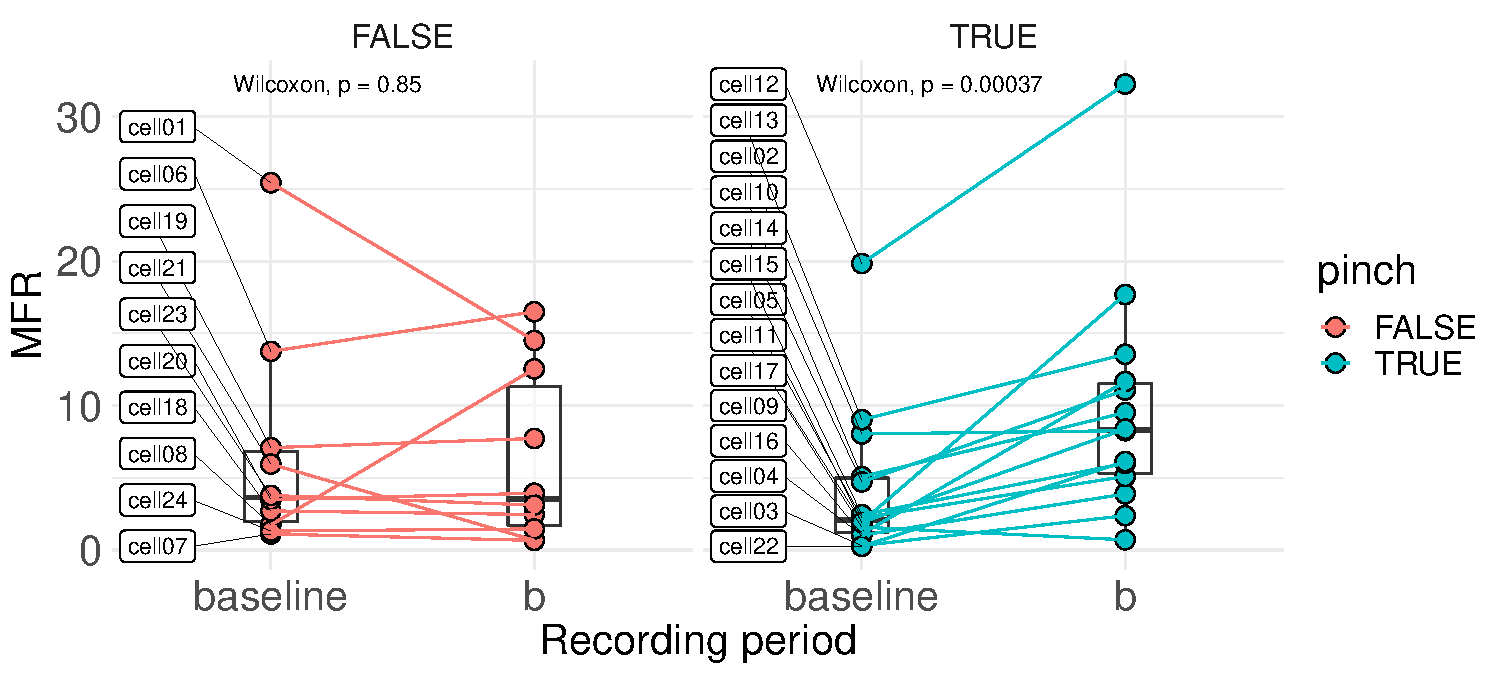
\includegraphics{GII_analysis_notebook_files/figure-latex/unnamed-chunk-13-1.pdf}

\hypertarget{mfr-before-during-and-after-stimulus}{%
\subsubsection{MFR before, during and after
stimulus}\label{mfr-before-during-and-after-stimulus}}

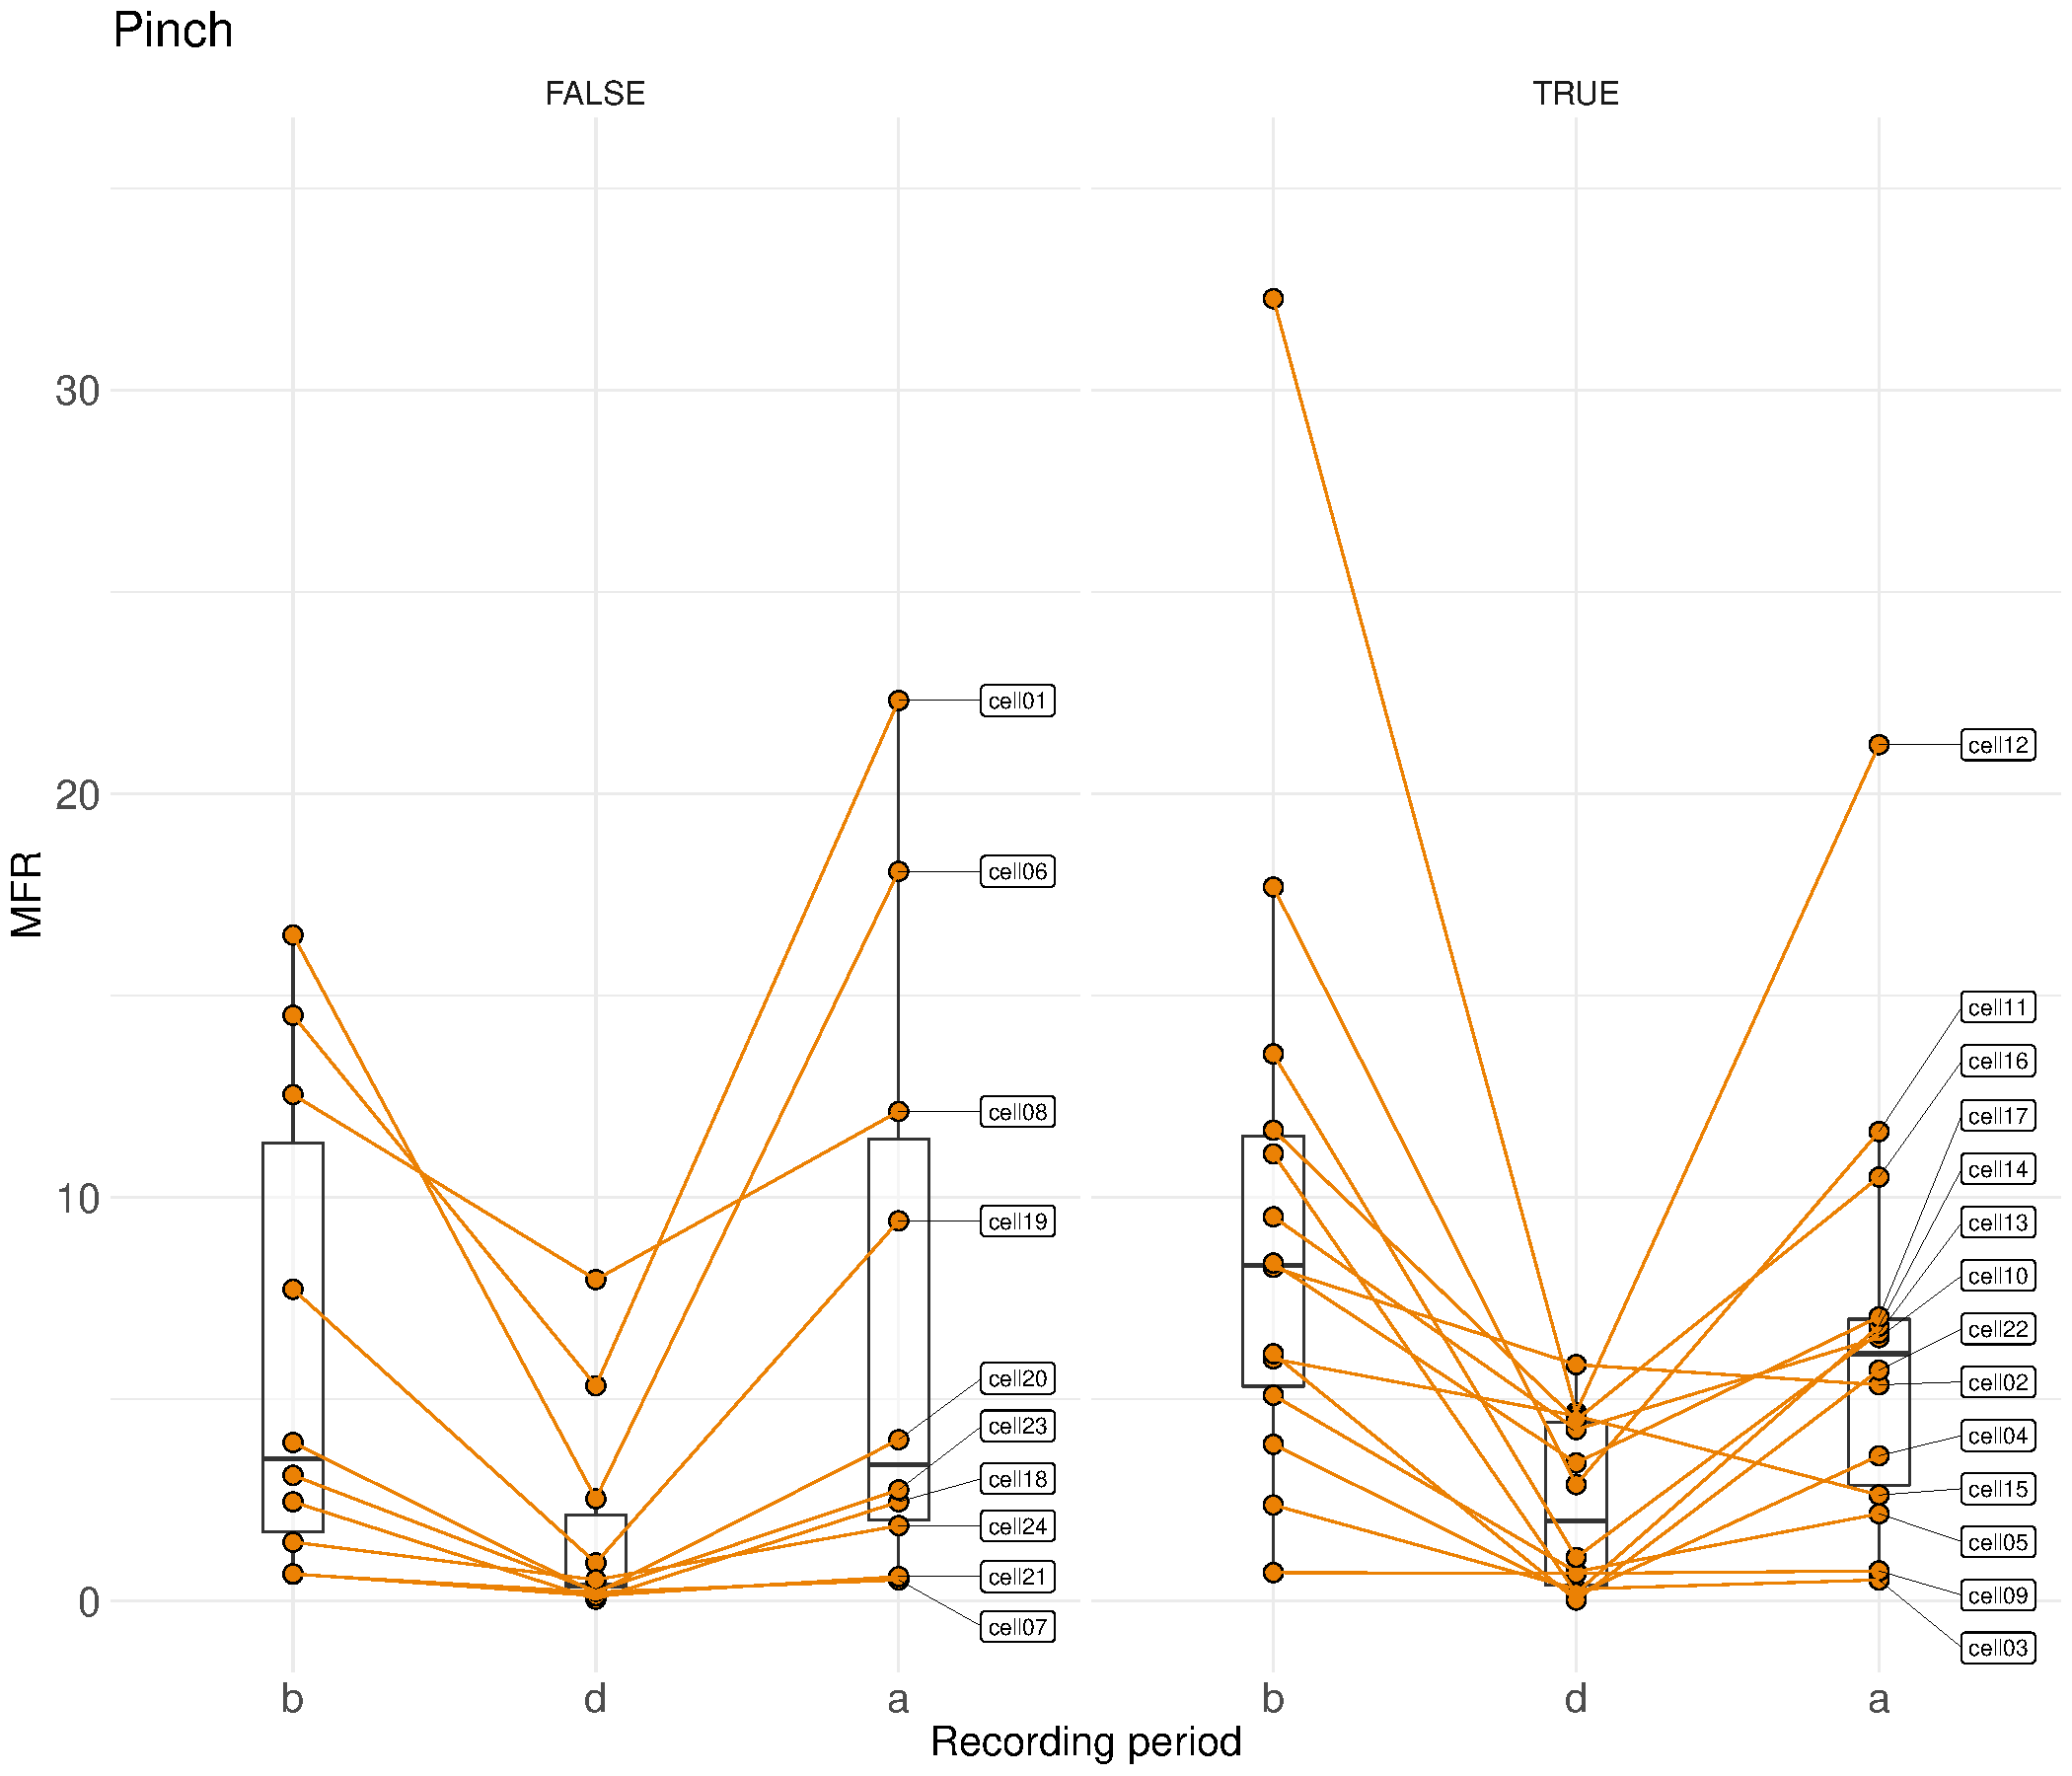
\includegraphics{GII_analysis_notebook_files/figure-latex/unnamed-chunk-14-1.pdf}

\hypertarget{strength-of-inhibition}{%
\subsubsection{Strength of inhibition}\label{strength-of-inhibition}}

Firing rate change \textbf{during} stimulus (photoactivation of the
glycinergic fibers) compared to \textbf{baseline}:

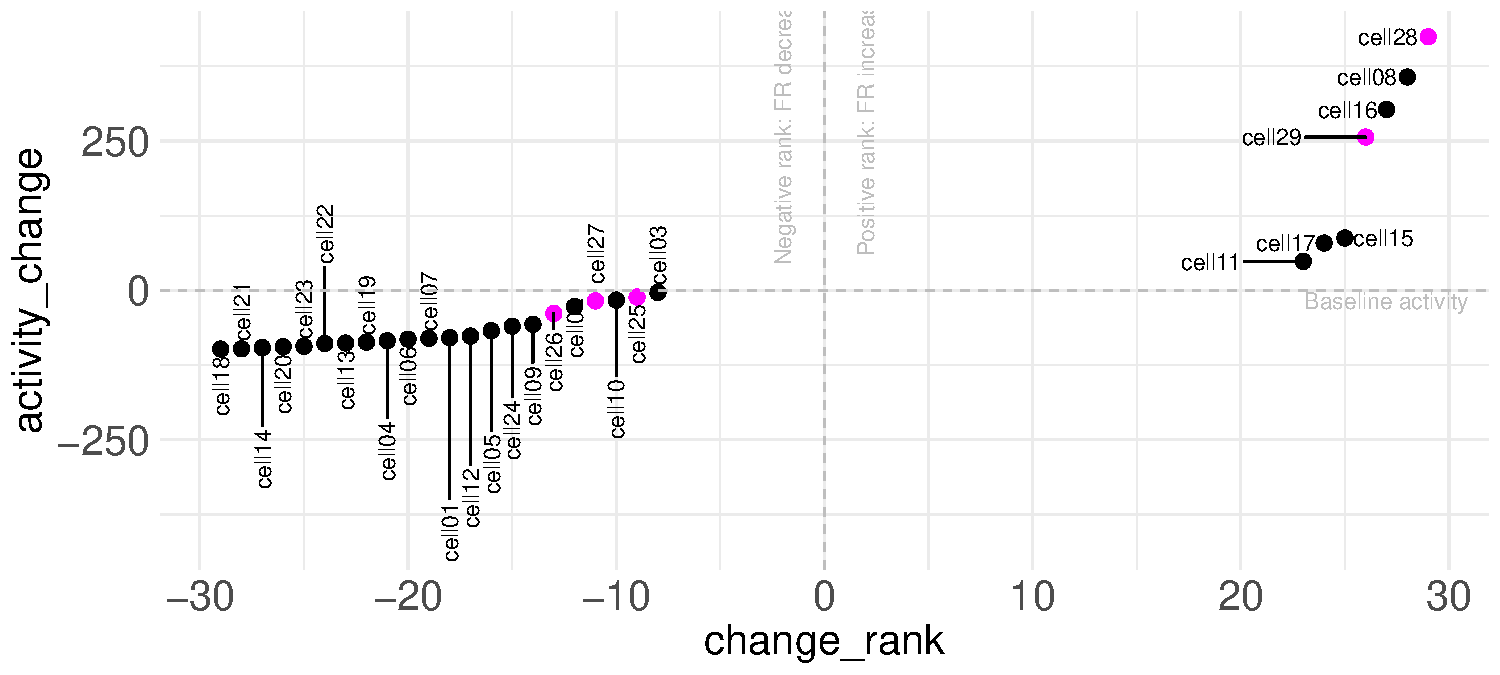
\includegraphics{GII_analysis_notebook_files/figure-latex/unnamed-chunk-15-1.pdf}

Firing rate change \textbf{during} stimulus (photoactivation of the
glycinergic fibers) compared to \textbf{before} stimulus:

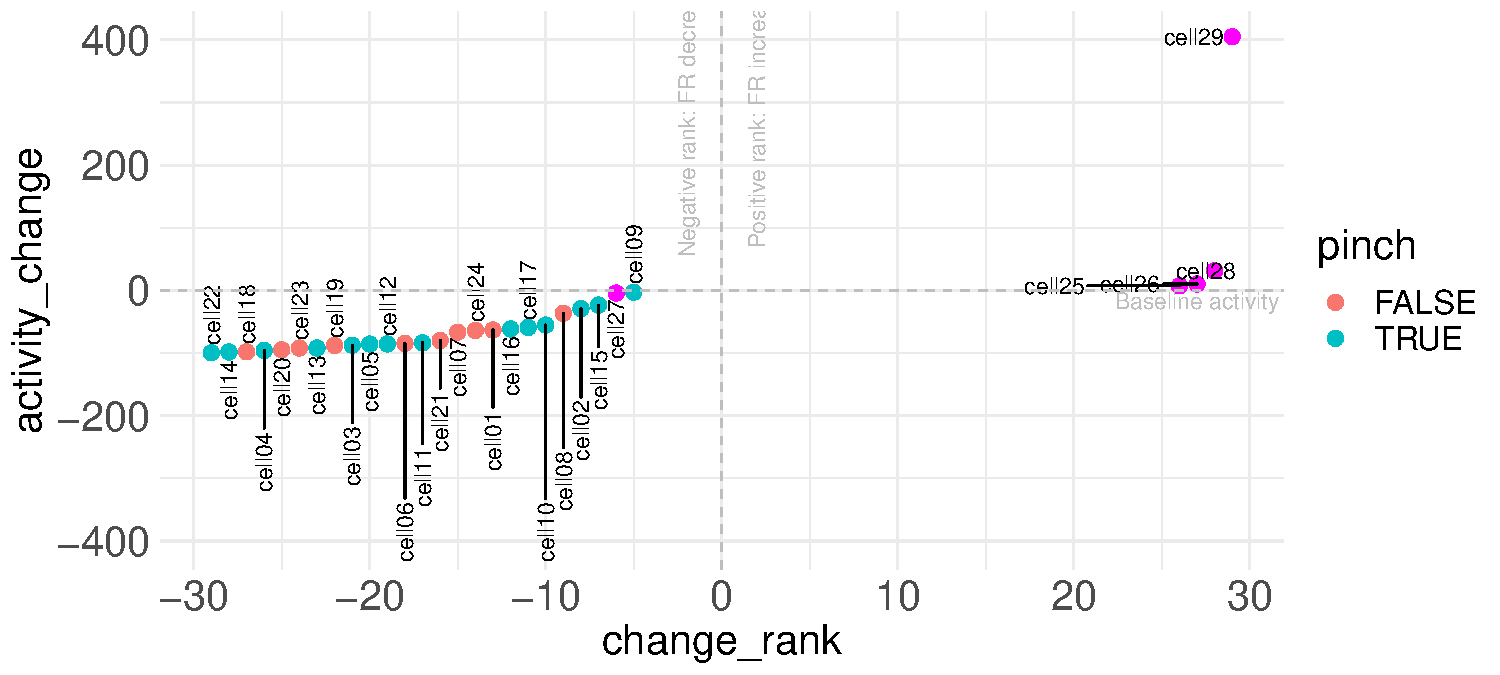
\includegraphics{GII_analysis_notebook_files/figure-latex/unnamed-chunk-16-1.pdf}

Plotting the change in MFR from ``\emph{baseline}'' to ``\emph{during
stimulus}''. Coloring based on the strength of the inhibition
(\emph{rank})

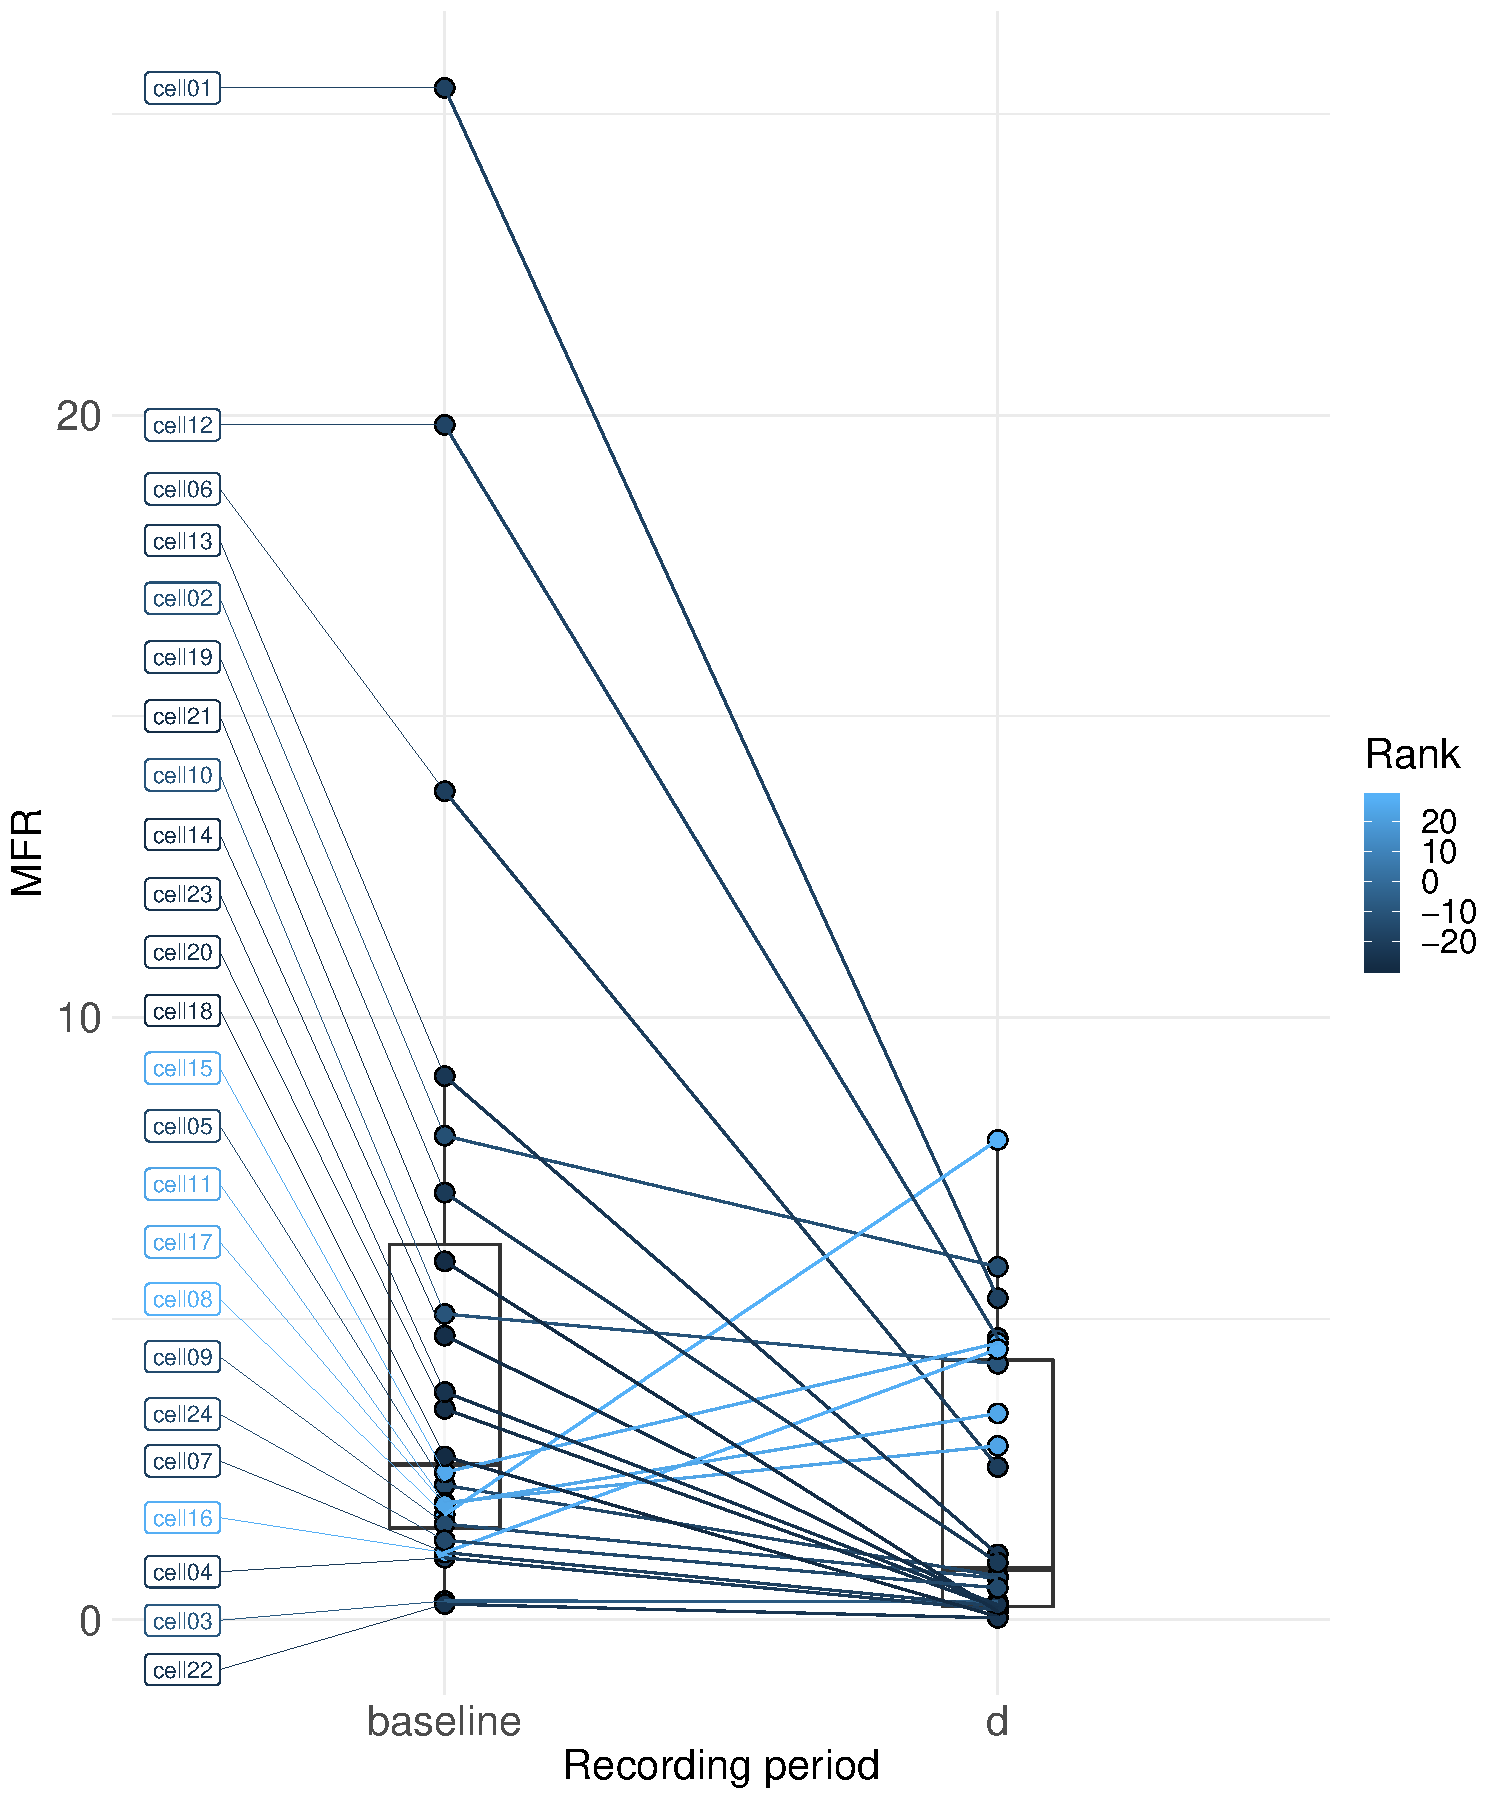
\includegraphics{GII_analysis_notebook_files/figure-latex/unnamed-chunk-17-1.pdf}

\hypertarget{activity-of-prf-glycinergic-cells-during-pfc-photoactivation}{%
\section{Activity of PRF glycinergic cells during PFC
photoactivation}\label{activity-of-prf-glycinergic-cells-during-pfc-photoactivation}}

\begin{itemize}
\tightlist
\item
  List of tibbles used to store data:

  \begin{itemize}
  \tightlist
  \item
    RECORDINGS tibble: stores AP and stim time stamps, number of stimuli
    in each train, stimulus frequency categories (eg. 8 10 and 12 Hz
    belong to 10 Hz category)
  \item
    STIM\_RESULTS: stores the data for PSTHs
  \end{itemize}
\end{itemize}

\begin{Shaded}
\begin{Highlighting}[]
\CommentTok{### adding stimulus number within}
\CommentTok{### train}
\NormalTok{RECORDINGS <-}\StringTok{ }\NormalTok{RECORDINGS }\OperatorTok\StringTok{ }\KeywordTok{mutate}\NormalTok{(}\DataTypeTok{stim_number =} \DecValTok{0}\NormalTok{)}

\CommentTok{### calculating stimulus number}
\CommentTok{### within train}
\NormalTok{initial_value <-}\StringTok{ }\NormalTok{RECORDINGS}\OperatorTok{$}\NormalTok{stim_freq[}\DecValTok{1}\NormalTok{] }\OperatorTok\StringTok{ }
\StringTok{    `}\DataTypeTok{comment<-}\StringTok{`}\NormalTok{(}\StringTok{"First value of stim_freq variable. When it changes stimulus counting restarts"}\NormalTok{)}

\NormalTok{stim_counter <-}\StringTok{ }\DecValTok{1} \OperatorTok\StringTok{ `}\DataTypeTok{comment<-}\StringTok{`}\NormalTok{(}\StringTok{"Counts stimuli in a train"}\NormalTok{)}
\NormalTok{index <-}\StringTok{ }\DecValTok{1} \OperatorTok\StringTok{ `}\DataTypeTok{comment<-}\StringTok{`}\NormalTok{(}\StringTok{"Tracks the position (index) of stim_freq"}\NormalTok{)}

\NormalTok{RECORDINGS}\OperatorTok{$}\NormalTok{stim_number[}\DecValTok{1}\NormalTok{] <-}\StringTok{ }\NormalTok{stim_counter}
\ControlFlowTok{repeat}\NormalTok{ \{}
    \ControlFlowTok{if}\NormalTok{ (RECORDINGS}\OperatorTok{$}\NormalTok{stim_freq[index }\OperatorTok{+}\StringTok{ }
\StringTok{        }\DecValTok{1}\NormalTok{] }\OperatorTok{==}\StringTok{ }\NormalTok{initial_value) \{}
\NormalTok{        RECORDINGS}\OperatorTok{$}\NormalTok{stim_number[index }\OperatorTok{+}\StringTok{ }
\StringTok{            }\DecValTok{1}\NormalTok{] <-}\StringTok{ }\NormalTok{stim_counter }\OperatorTok{+}\StringTok{ }
\StringTok{            }\DecValTok{1}
\NormalTok{        stim_counter <-}\StringTok{ }\NormalTok{stim_counter }\OperatorTok{+}\StringTok{ }
\StringTok{            }\DecValTok{1}
\NormalTok{        index <-}\StringTok{ }\NormalTok{index }\OperatorTok{+}\StringTok{ }\DecValTok{1}
\NormalTok{    \} }\ControlFlowTok{else}\NormalTok{ \{}
\NormalTok{        initial_value <-}\StringTok{ }\NormalTok{RECORDINGS}\OperatorTok{$}\NormalTok{stim_freq[index }\OperatorTok{+}\StringTok{ }
\StringTok{            }\DecValTok{1}\NormalTok{]}
\NormalTok{        stim_counter <-}\StringTok{ }\DecValTok{1}
\NormalTok{        RECORDINGS}\OperatorTok{$}\NormalTok{stim_number[index }\OperatorTok{+}\StringTok{ }
\StringTok{            }\DecValTok{1}\NormalTok{] <-}\StringTok{ }\NormalTok{stim_counter}
\NormalTok{        index <-}\StringTok{ }\NormalTok{index }\OperatorTok{+}\StringTok{ }\DecValTok{1}
\NormalTok{    \}}
    
    \ControlFlowTok{if}\NormalTok{ (index }\OperatorTok{==}\StringTok{ }\KeywordTok{length}\NormalTok{(RECORDINGS}\OperatorTok{$}\NormalTok{stim_number)) \{}
        \ControlFlowTok{break}
\NormalTok{    \}}
\NormalTok{\}}
\end{Highlighting}
\end{Shaded}

\hypertarget{spontaneous-desynchronization-of-the-fc-slow-oscillation}{%
\section{Spontaneous desynchronization of the FC slow
oscillation}\label{spontaneous-desynchronization-of-the-fc-slow-oscillation}}

\begin{Shaded}
\begin{Highlighting}[]
\NormalTok{file_to_load <-}\StringTok{ }\NormalTok{file_list[[}\DecValTok{1}\NormalTok{]]}
\NormalTok{filename <-}\StringTok{ }\KeywordTok{as.character}\NormalTok{(}\KeywordTok{substring}\NormalTok{(file_to_load, }
    \DecValTok{1}\NormalTok{, }\KeywordTok{nchar}\NormalTok{(file_to_load) }\OperatorTok{-}\StringTok{ }\DecValTok{4}\NormalTok{))}
\NormalTok{raw.rec <-}\StringTok{ }\KeywordTok{readMat}\NormalTok{(}\KeywordTok{file.path}\NormalTok{(}\StringTok{"data"}\NormalTok{, }
\NormalTok{    file_to_load))}

\CommentTok{### takes the first AP (first}
\CommentTok{### row) and tells the index of}
\CommentTok{### point with the max value}
\NormalTok{points_to_peak <-}\StringTok{ }\KeywordTok{which}\NormalTok{(raw.rec}\OperatorTok{$}\NormalTok{ap[, }
\NormalTok{    , }\DecValTok{1}\NormalTok{]}\OperatorTok{$}\NormalTok{values[}\DecValTok{1}\NormalTok{, ] }\OperatorTok{==}\StringTok{ }\KeywordTok{max}\NormalTok{(raw.rec}\OperatorTok{$}\NormalTok{ap[, }
\NormalTok{    , }\DecValTok{1}\NormalTok{]}\OperatorTok{$}\NormalTok{values[}\DecValTok{1}\NormalTok{, ])) }\OperatorTok\StringTok{ }\KeywordTok{as.numeric}\NormalTok{()}

\CommentTok{### time of the peak of the APs}
\CommentTok{### after its first point}
\NormalTok{raw.rec}\OperatorTok{$}\NormalTok{ap[, , }\DecValTok{1}\NormalTok{]}\OperatorTok{$}\NormalTok{interval }\OperatorTok{*}\StringTok{ }\NormalTok{points_to_peak}
\end{Highlighting}
\end{Shaded}

\begin{verbatim}
##         [,1]
## [1,] 0.00055
\end{verbatim}

\begin{Shaded}
\begin{Highlighting}[]
\NormalTok{ap <-}\StringTok{ }\NormalTok{raw.rec}\OperatorTok{$}\NormalTok{ap[, , }\DecValTok{1}\NormalTok{]}\OperatorTok{$}\NormalTok{times }\OperatorTok\StringTok{ }
\StringTok{    }\KeywordTok{as.double}\NormalTok{()}
\NormalTok{ap_peaks <-}\StringTok{ }\KeywordTok{tibble}\NormalTok{(}\DataTypeTok{peak_times =}\NormalTok{ (ap }\OperatorTok{+}\StringTok{ }
\StringTok{    }\KeywordTok{c}\NormalTok{(raw.rec}\OperatorTok{$}\NormalTok{ap[, , }\DecValTok{1}\NormalTok{]}\OperatorTok{$}\NormalTok{interval }\OperatorTok{*}\StringTok{ }
\StringTok{        }\NormalTok{points_to_peak)))}
\end{Highlighting}
\end{Shaded}

------- insert code here --------

(spont\_desynchron\_analysis.R), 7 recordings


\end{document}
